\maketitle

\begin{abstract}
In the life-cycle of objects there are different phases. The phase in which an object currently is, affects how it is handled in an application; however phase shifts are typically implicit.
In this study we propose an extension to the aspect-oriented language AspectJ with a new mechanism, called \emph{instance pointcuts}, for creating and maintaining categories of objects according to events in their life-cycle; these events are selected with pointcut-like specifications.


The selection criteria of instance pointcuts can be refined, e.g., by restricting the scope of an existing instance pointcut; and they can be composed, e.g., by boolean operations.
We offer a means to access all objects currently selected by an instance pointcut from Java code, i.e., to be used in methods or advice bodies; and we expose the events of adding or removing an object from an instance pointcut by creating a join point that can be selected by regular pointcuts.
Our approach improves modularity by providing a fine-grained mechanism and a declarative syntax to define and maintain object categories.
\end{abstract}

% A category with the (minimum) three required fields
\category{D.3.1}{Formal Definition and Theory}[syntax, semantics]
%A category including the fourth, optional field follows...
\category{D.3.4}{Processors}[code generation]

\section{Introduction}
In object-oriented programming (OOP), objects encapsulate state and behavior; objects also have a life-cycle, which means that the same object can play different roles at different times.
Which role an object is currently playing can affect the object's own behavior or how it is handled.
Typically the shift from one life-cycle phase to another is implicitly marked by events, e.g., passing an object from one client to another.

As an example of relevant phases in the life-cycle of objects, consider an online store application with ``vendor'' objects representing the suppliers and ``product'' objects representing the products they sell. 
Assume we would like to keep the list of products which were applied the happy-hour discount. Each product is assigned to a different time slot as its happy-hour, so the list of products that are discounted is changing over time. 
Categorizing objects according to criteria that is not directly supported by the programming language, such as which class they were initialized in, which method they were passed to as an argument, or (as in the example) the time at which they are passed to a method, requires invasively inserting bookkeeping code.

Aspect-oriented programming can be applied to separate this bookkeeping code from the business logic of the program. But in AOP, \emph{pointcuts} select sets of so-called \emph{join points} which are points in time during the execution of the program. Current aspect-oriented languages do not support a \emph{declarative specification} of the objects belonging to a life-cycle phase; instead an \emph{imperative implementation}, always following the same pattern, is required for collecting those objects.
A consequence of such an imperative solution is reduced readability and maintainability due to boilerplate code.


To offer better support for processing objects according to their life-cycle phase, we propose a new mechanism, called \emph{instance pointcuts}, to select sets of objects based on the events in their execution history.
Instance pointcuts are used to declare the beginning and the end of a life cycle as events. Instance pointcuts can be reused via refinement and composition operations and their implementation provides checks to ensure correctness. 

An instance pointcut's concise definition consists of three parts: an identifier, a type which is the upper bound for all objects in the selected set, and a specification of relevant objects.
The specification utilizes \emph{pointcut expressions} to select events that define the begin and end of life-cycle phases and to expose the object. At these events, an object is added or removed from the set representing the instance pointcut. 
New instance pointcuts can be derived from existing ones. Firstly, a new instance pointcut can be derived from another one by restricting the type of selected objects. 
Secondly, instance pointcut declarations can be composed arbitrarily by means of set operators. 
The declarative nature of instance pointcuts allow several checks to be performed which are not automatically possible with equivalent imperative code. Such checks are important to notify the developer about empty sets, ill-formed composition expressions,  illegal instance pointcut compositions and refinements, etc.  These checks ensure the correctness of the instance pointcuts and consistence in object categories. 

In this paper we present instance pointcuts as an extension to AspectJ \cite{kiczales2001overview} and explain its semantics by explaining our compiler which transforms instance pointcuts to plain AspectJ and advanced dispatching library calls. 

The rest of the paper is organized as follows, in section~\ref{sect:motivation} we present a small case study and explain our motivation for the proposed approach. In section~\ref{sect:ip} a detailed description of instance pointcuts and its various features are presented. This section also explains how instance pointcuts are compiled. We then present a discussion on the validation of our approach. We conclude by discussing related work and giving a summary of our approach.


\section{Motivation}
\label{sect:motivation}

Objects can be categorized by how they are used (passed as arguments to method calls, act as receiver or sender for method calls, etc.) and concerns of an application may be applicable only to objects used in a specific way.
Therefore we must be able to identify and select those objects.
We want to expose sets of objects belonging to the same category by means of a dedicated language construct such that the implementation of phase-dependent concerns can explicitly refer to the category.

\begin{figure*}
\centering
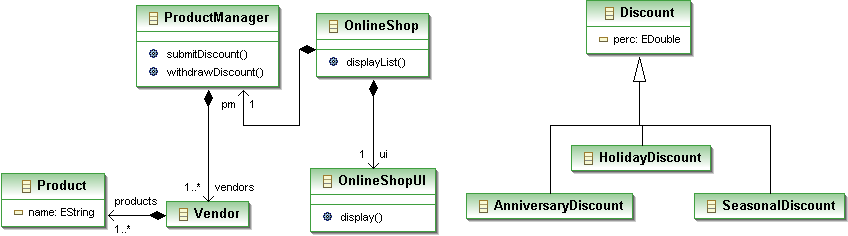
\includegraphics[width= 0.75\textwidth]{images/onlineshop2.png}%
\vspace{10pt}
\caption{Part of an online shop application}%
\label{fig:shop}%
\end{figure*}

In Figure~\ref{fig:shop}, we outline a part of the architecture of an online store application from the \emph{system's perspective}. We use this scenario to give examples of categorizing objects according to how they are used and how to use these categories in the implementation of concerns. It must be noted that we intend to support the addition of \emph{unanticipated} concerns, i.e., the program code is not prepared to support abstractions, like specific object categories, required by the new concerns. 
%At the end of this section, we conclude requirements for solving the encountered challenges in these examples.

\subsection{Example Architecture}
An online shop is a sophisticated web application and objects of the same type can exist at different stages of their life-cycle. In Figure~\ref{fig:shop} the static structure of a simplified online shop is shown. This structure shows part of the system from the \lstinln{Vendor} and the \lstinln{OnlineShop}'s perspective. \lstinln{Vendor}s can submit different kinds of \lstinln{Discount}s to the \lstinln{ProductManager} for the \lstinln{Product}s they are selling. \lstinln{Product} is the root of the type hierarcy and is parent to the types such as \lstinln{BeautyProduct}, \lstinln{SportProduct}~\dots(Not shown in the figure). Each \lstinln{Product} holds a list of \lstinln{Discounts} they are applied. The \lstinln{OnlineShop} has a user interface represented by the \lstinln{OnlineShopUI} class, which is used to display information to the customers. 


\subsection{Unanticipated Extensions}
A new feature is added to the online shop which requires creating an alert when a product is applied a surprise discount, also the list of surprise discounted products should be available to the user at any time. The surprise discounts are submitted by \lstinln{Vendor}s and they can be submitted or withdrawn any time.  In order to realize this extension in an OO-approach, we need to change several classes to host this extension. First the class \lstinln{ProductManager} should keep a set of \lstinln{Product}s which are applied a surprise discount, in Listing~\ref{lst:discountalert} this is shown in line~\ref{surpdisset}. This set is updated when a new discount of type \lstinln{SurpriseDiscount} is submitted or withdrawn (lines~\ref{surpset:begin}--~\ref{surpset:end}). There should also be some changes in the \lstinln{OnlineShop} class. First a \lstinln{createDiscountAlert} method should be added. Also the \lstinln{displayList} method should be updated to include the \lstinln{surpriseDiscount} list defined in the \lstinln{ProductManager} class.


\begin{lstlisting}[float, caption={A Java implementation of discount alert concern}, label={lst:discountalert}]
class ProductManager{
	...
	~\bh~Set<Product> surpriseDiscount = createSet(); ~\eh\label{surpdisset}~
	public void submitDiscount(Product p, Discount d)~\label{surpset:begin}~
	{
		...
		if(d instanceof SurpriseDiscount)
		{
			surpriseDiscount.add(p);
			OnlineShop.createDiscountAlert(p);
		}
	}
	public boolean withdrawDiscount(Product p, Discount d)
	{
		...
		if(d instanceof SurpriseDiscount)
			surpriseDiscount.remove(p);
	}~\label{surpset:end}~
}
class OnlineShop{//SINGLETON
	...
	public void createDiscountAlert(Product p)
	{
		//create surprise discount alert for p
	}
	public void displayList(String listType)
	{
		if(listType.equals(``surprise'')
			INSTANCE.getUI().display(ProductManager.surpriseDiscount);
	}
}
\end{lstlisting}


The OO-solution is scattered among \lstinln{ProductManager} and \lstinln{OnlineShop} classes and tangled with multiple methods. The code for the surprise discount concern and the book-keeping that comes with it creates cluttering. 
An aspect-oriented implementation can offer a better solution by encapsulating the concern in an aspect. 
In Listing~\ref{lst:discountaop} shows a possible solution. The set of products which are applied a surprise discount is kept in the aspect (line~\ref{daop:set}). The following two pointcuts \lstinln{submit} and \lstinln{withdraw} selects the products to which a \lstinln{SurpriseDiscount} is applied (lines~\ref{daop:pc:submit}--~\ref{daop:pc:wdraw}). The corresponding advice declarations for these pointcuts maintain the \lstinln{surpriseDiscount} set, also the \lstinln{submit} join-point triggers the surprise discount alert method (line~\ref{daop:alert}). There is also the \lstinln{display} pointcut (line~\ref{daop:pc:display}, which intercepts the call to \lstinln{displayList} method and add the condition for the surprise discount list in an around advice (lines~\ref{daop:around:begin}--~\ref{daop:around:end}). This aspect also includes an inter-type declaration which adds the \lstinln{createDiscountAlert} method to the \lstinln{OnlineShop} class.


\begin{lstlisting}[float=h, caption={An Aspectj implementation of discount alert concern}, label={lst:discountaop}]
~\hilight~Set<Item> surpriseDiscount = createSet();~\label{daop:set}~
~\hilight~pointcut submit(Product p): call(* ProductManager.submitDiscount(..)) && args(p, SurpriseDiscount); ~\label{daop:pc:submit}~
~\hilight~pointcut withdraw(Product p): call(* ProductManager.withdrawDiscount(..)) && args(p, SurpriseDiscount); ~\label{daop:pc:wdraw}~
pointcut display(String listType): call(* OnlineShop.displayList(..)) && args(listType);~\label{daop:pc:display}~
after(Product p): submit(p){
	~\hilight~surpriseDiscount.add(p);
	OnlineShop.instance().createDiscountAlert(p);~\label{daop:alert}~
}
after(Product p):withdraw(p){
	~\hilight~if(surpriseDiscount.contains(p))
		~\hilight~supriseDiscount.remove(p);}
}
void around(String listType):display(listType){~\label{daop:around:begin}~
	if(listType.equals(``surprise'')
		OnlineShop.instance().getUI().display(surpriseDiscount);
	proceed(listType);	
} ~\label{daop:around:end}~
public void OnlineShop.createDiscountAlert(Product p){
	//create surprise discount alert for a product
}
\end{lstlisting}

\paragraph{Discussion and Requirements}

AOP already helps to localize the concern and to add it without the need to modify existing code.
%But most of the implementation of the surprise discount concern as shown in Listing~\ref{lst:discountaop} consists of boilerplate code .
However maintenance of the \lstinln{surpriseDiscount} set requires the same boilerplate code the OO solution does (highlighted in gray).
Essentially what the code does is select \lstinln{Product} objects based on the discount they are applied to and deselect them once they are rid of this discount. 
This marks a phase in the life-cycle of a \lstinln{Product} object, none of the presented solutions offer any declarative means to define such a life-cycle phase.
Furthermore, reusing such existing sets by refining or composing them is not conveniently supported at all; e.g., if we want to find the subset of \lstinln{BeautyProduct}s of the \lstinln{surpriseDiscount} set, we have to iterate over it and check instance types to create a new set. This iterative way of refining does not give us any informationabout the set being empty or populated; this kind of a check also needs additional code. From this motivating example we conclude our problem statement as follows.

\paragraph{Problem Statement}
Creating objects sets according to execution events is a crosscutting concern. Current programming approaches only provide imperative ways to maintain object sets which result in code that is marginally concern-specific and majorly boilerplate. The maintenance costs of such programs hinder software evolution and their imperative nature prevents useful checks.







%\begin{enumerate}[{Requirement}1{:}]
%\item A declarative way of reifying a set of objects by defining add/remove conditional expressions must be provided.
%\item Since objects may recursively enter and exit a life-cycle phase, it must be counted how often the begin and end events have occurred for each object.
%\item Add/Remove expressions must select events and specify which object from the context of the event is selected.
%\item It must be possible to access the set of objects which currently comprises an object category and to be notified when the set changes.
%\item A declarative way to obtain new sets by composing existing ones is required.
%\item Validity should be ensured for composition, either by construction or through compile-time checks.
%\end{enumerate}
